\documentclass[12pt, a4paper]{article}
\usepackage[margin=1.3in]{geometry}
\usepackage{tikz}
\usepackage{graphics}
\usepackage{amsmath}
\usepackage{subfig}

% Title Page
\title{Evolving Tower-Destroying Robots\\\normalsize An Exploration into Scaffolded Learning}
\author{Ryan Boldi}


\begin{document}
\maketitle
\tableofcontents
\newpage
\section{Goals}
We do not teach linear algebra to 6 year olds due to the fact that they do not have sufficient educational \emph{scaffolding} to grasp such a bizarre concept. My goal was to see whether or not this also applies to a robot evolving to do a certain task.\par 
The robot's task is to destroy a tower that starts a specific distance away from it:\par
\vspace{-10pt}
\begin{figure}[h]
	
\begin{center}
	\centering
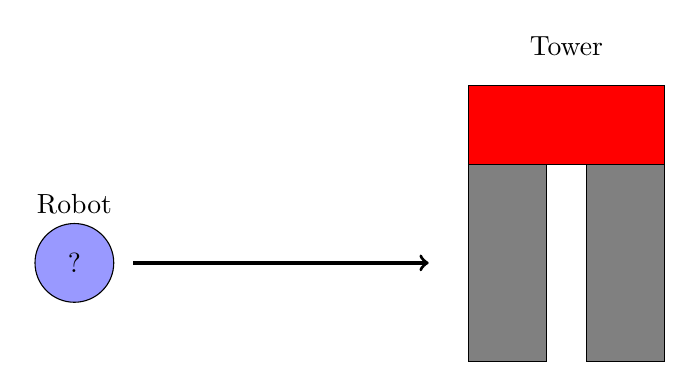
\begin{tikzpicture}
\filldraw[fill=blue!40!white](0,1.25) circle (5mm);
\node[] at (0,1.25) {?};
\node[] at (0,2) {Robot};
\draw [->, very thick] (0.75, 1.25) -- (4.5,1.25);
\filldraw[fill=gray] (5,0) rectangle (6,2.5);
\filldraw[fill=gray](6.5,0) rectangle (7.5,2.5);
\filldraw[fill=red] (5,2.5) rectangle (7.5,3.5);
\node[] at (6.25,4) {Tower};
\end{tikzpicture}
\caption{Diagram demonstrating the robot's task.}
\label{goal}
\end{center}
\end{figure}
\vspace{-10pt}
To scaffold the learning of the robot, I planned to start the tower close to the robot, and slowly move it farther and farther away over the course of many generations. This will continue until the tower is at the goal distance from the robot. These are environmental changes that starts the robot with an easy task, waits for the task to be complete, then makes the task slightly harder. This process is repeated until the robot has mastered the most difficult goal task.\par
My goal was to experiment with this process, seeing whether or not it actually improved the speed of solution discovery, or quality of the solutions themselves.
\newpage

\section{Implementation}
\paragraph{Robot}
I started by creating the robot. It was based on a simple quadruped, but with 2 added arms to make destroying the tower easier. All of the limb relative sizes can be controlled and fined tuned in \emph{constants.py}.\par
\begin{figure}[h]
	\centering
	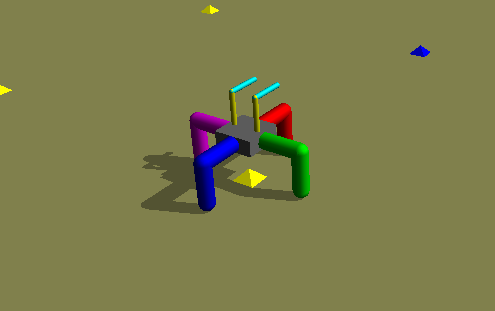
\includegraphics{robot.png}
	\caption{The \emph{Tower-Destroyer} Robot. It has 6 sensors: one on the tip of each limb. It may move its legs and arms freely, each with 2 degrees of freedom. Each motor is controlled by the output layer of a fully connected neural network, which takes the sensor data as inputs. }
\end{figure}
\paragraph{Tower}
The Tower is created out of 3 similar cuboids, with the third balanced on top of the bottom two (see figure~\ref{goal}). The block colored in red is to be my `fall detector'. If this block comes into contact with the ground, we will count this tower as ``Fallen". If the tower has fallen over, the robot will receive a large fitness reward.
\paragraph{Fitness} To ensure that the reinforcement is not too sparse, I wanted to include an incentive to move towards the tower. After much deliberation, this is the fitness function I have included:
$$
\text{Fitness} = \begin{cases}
\text{distance from origin}_y & \text{if tower did not fall};\\
20 & \text{if tower fell.}\\
\end{cases}
$$

\noindent I believed that this would promote movement in the positive $y$ direction before the tower is in the robot's reach.

\paragraph{Scaffolding} To control whether or not we are going to scaffold the robot's learning, I added a new constant to the program that controls how many generations of \emph{pretraining} will occur. During pretraining, the tower's distance starts at low value, and incrementally gets larger as the robot performs better. When these pretraining generations are completed, the tower's distance will be set to the maximum (goal) distance, and the evolution continues until all of the total generations have completed. If pretraining is set to 300, and total generations is set to 600, we will pretrain the population for 300 generations, slowly incrementing the tower's distance whenever a robot successfully knocks over the tower. At 300 generations, no matter the current distance of the tower, we move it to it's maximum distance for the final 300 generations. If pretraining is set to 0, and total generations is set to 600, we will start the tower at its maximum distance, and train the population on that for 600 generation without moving the tower.
\newpage
\section{Results}
I expected that the robots that were pretrained in the simpler environment would do better than robots that were solely trained on the difficult environment. If this was the case, we would see the robots that have been pretrained for half of the total evolutionary time do better in that second half where they are in the difficult environment. This provides us with a fair means of comparison between the two evolutionary methods. 
\begin{figure}[h]
	\centering
	\title{No Pretrain, 600 Total}
	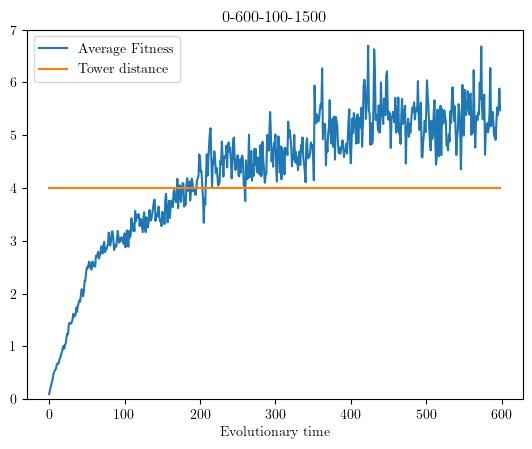
\includegraphics[width=1\textwidth]{0-600-100-1500/0-600-100-1500.png}
	\caption{Result after 100 robots were evaluated for 1500 timesteps per generation, over the course of 600 generations, 0 of which are pretraining. Because there was no pretraining, the tower stays at a constant distance away from the robot over the entire course of evolution. The fitness of the robots is their distance from the origin in the $y$ direction, so the point where the blue and orange lines meet effectively represents when the robots reach the tower. Past this, the only way to get fitness is to destroy the tower, which is how the fitness continues to increase.}
	\label{nopretrain}
\end{figure}

Figure~\ref{nopretrain} proves that evolution did in fact take place. We can see that the evolved creatures do much better than the randomly evolved creatures in generation 0.

Next, I repeated evolution, but set pretrain to 300. This means that half of evolution will take place in the pretrain phase, where the tower gets incrementally farther away, until generation 300, where the tower is set to its maximum distance.

%discuss that this was what i expected, eventually, due to the fact that i give them inentive to move forward, the robots will learn to walk towards the tower, and one of them will eventually break down the tower.
%in the future, i could maybe vary where the tower is, so that the creatures that train on the closer towers have an easier time when it gets further away


\begin{figure}[h]
\centering
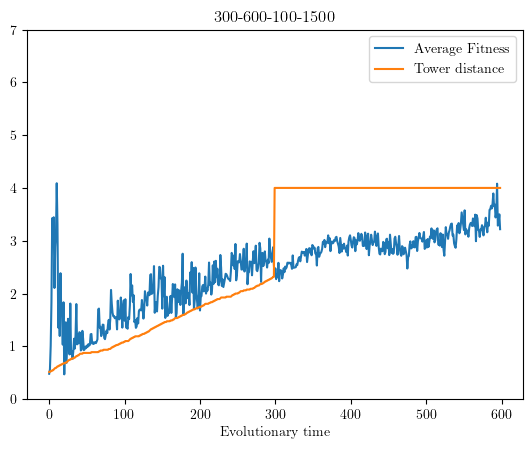
\includegraphics[width=1\textwidth]{300-600-100-1500/300-600-100-1500.png}
\caption{Result after 100 robots were evaluated for 1500 timesteps per generation, over the course of 600 generations of evolution, 300 of which are pretraining. We can see that the robots are able to destroy the tower at the beginning, but as the tower gets farther away they are less able to do so. We can see that after 300 generations, none of the robots are able to knock over the tower as it is at its maximum offset of 4. There is a large spike of fitness at the beginning due to how easy it is to destroy the tower (just falling forward). Only in one of the last generations was a robot able to knock over the tower (because the blue line is above the orange line, therefore the average fitness is larger than the distance to the tower).}
\end{figure}
\newpage
\begin{figure}[h]
	\centering
	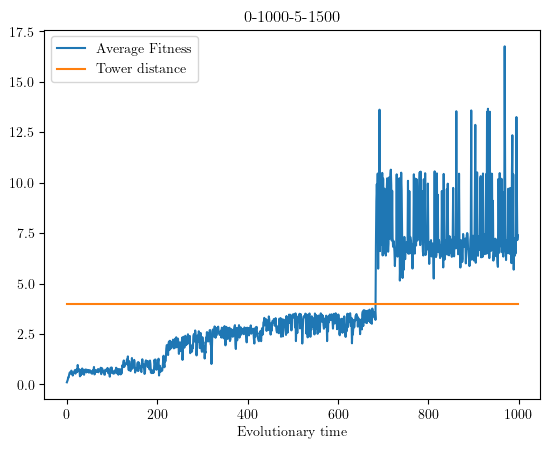
\includegraphics[width=\textwidth]{0-1000-5-1500/0-1000-5-1500.png}
	\caption{Result after 5 robots were evaluated for 1500 timesteps per generation, over the course of 1000 generations of evolution, 0 of which are pretraining.}
	\label{0-1000-5}
\end{figure}

\begin{figure}[h]
	\centering
	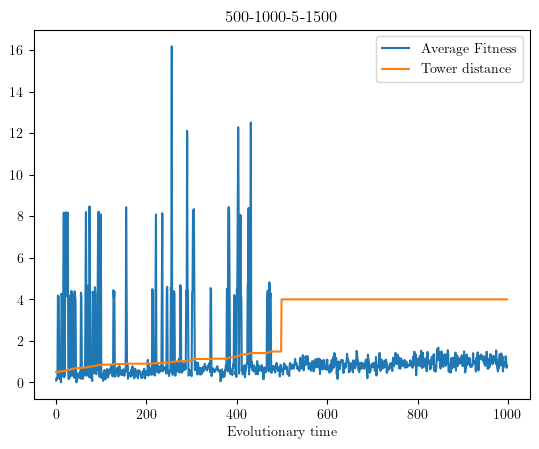
\includegraphics[width=1\textwidth]{500-1000-5-1500/500-1000-5-1500.png}
	\caption{Result after 5 robots were evaluated for 1500 timesteps per generation, over the course of 1000 generations of evolution, 500 of which are pretraining.}
	\label{500-1000-5}
\end{figure}

After repeating the experiment with less creatures and more generations, we see results that are consistent with the earlier run. Figures~\ref{0-1000-5} and~\ref{500-1000-5} show that pretraining is adversely affecting evolution. We can tell that this is the case because the evolutionary run without pretraining yields a solution that can destroy the tower at its maximum distance of 4. Yet, with pretraining, the robots do not destroy the tower at all when it is at its maximum distance. As shown in figure~\ref{0-1000-5}, it took around 700 generations for a robot controller to be discovered that can destroy the tower. But, with pretraining, no robot comes close to destroying the tower for portion of evolution where the tower is at 4 units away.

To ensure that these results were not just coincidences, I ran evolution one more time, and gave the pretraining many more generations to help smoothen the transition from pretrianing to regular evolution.

\begin{figure}[h]
	\centering
	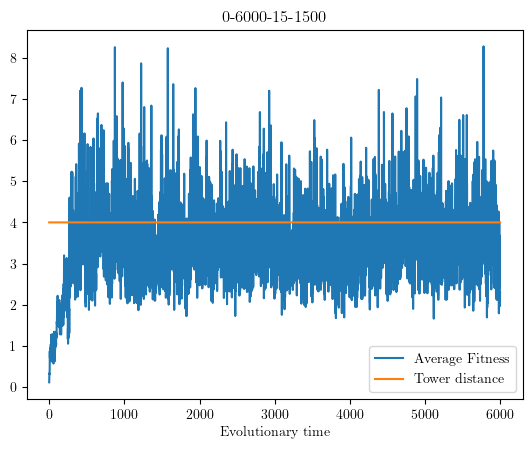
\includegraphics[width=1\textwidth]{0-6000-15-1500/0-6000-15-1500.png}
	\caption{Result after 5 robots were evaluated for 1500 timesteps per generation, over the course of 1000 generations of evolution, 500 of which are pretraining.}
	
\end{figure}
\begin{figure}[h]
	\centering
	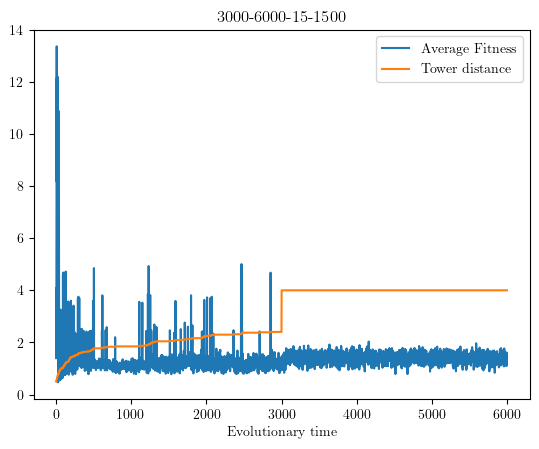
\includegraphics[width=1\textwidth]{3000-6000-15-1500/3000-6000-15-1500.png}
	\caption{Result after 5 robots were evaluated for 1500 timesteps per generation, over the course of 1000 generations of evolution, 500 of which are pretraining.}
	
\end{figure}

\section{Reflection}

\end{document}          
